\documentclass[10pt]{article}
\usepackage{amsmath}
\usepackage[english,catalan,spanish]{babel}
\usepackage{ucs}
\usepackage[utf8]{inputenc}
\usepackage[T1]{fontenc}
\usepackage{float}
\usepackage{textcomp}
\usepackage{graphicx}
\usepackage[usenames,dvipsnames,svgnames,table]{xcolor}
\usepackage{url}
\usepackage{fancyhdr}
% Permite emplear cualquier medida de márgenes.
\usepackage{anysize}
\setlength{\parindent}{0cm}
% Controla los márgenes {izquierda}{derecha}{arriba}{abajo}. 
\marginsize{3cm}{2cm}{2cm}{3cm}
%\topmargin=-3cm
%\leftmargin=-3cm
%\setlength{\textheight}{250mm}
\pagestyle{fancy}
\newcommand{\HRule}{\rule{\linewidth}{0.5mm}}
\newcommand{\titol}{\textcolor{red}}
\newcommand{\enunciat}{\textbf}
\author{}
\title{}
\setlength{\parindent}{0cm}
\date{\today}
\selectlanguage{catalan}
%\setlength{\topmargin}{-2 cm}
\begin{document}
\begin{titlepage}
%\setlength{\topmargin}{-1 cm}
\begin{center}
\LARGE{Introduction to PERL\\ Master in Bioinformatics for Public Health }\\
\end{center}

\vspace{4.5cm}

\HRule \\[0.4cm]
\begin{center}
{ \Huge \bfseries Getting the Topmost Scoring Sequences from Position Weight Matrices \\[0.8cm] }
\end{center}
\HRule \\[0.4cm]

\vspace{4.5cm}
\begin{center}
\huge{Joan Francesc Gilabert Navarro}\\
\vspace{0.5cm}
\begin{LARGE}
\today
\end{LARGE}
\end{center}
\end{titlepage}
\newpage
\section{Algorithm}

To generate the n-topmost scoring sequences from a position-weight matrix (PWM) we propose an algorithm divided in tow blocks:
\begin{enumerate}
\item Pre-processing of PWM
\item Sequence generation
\end{enumerate}

\subsection{Pre-processing of PWM}

The PWM can be rearranged to a more advantageous ordering, with the columns ordered by the top-scoring nucleotides and the row ordered by the smallest change between the first and second top-scoring nucleotides in that same row. This ordering allows us to trivially generate the top-scoring sequence, which is the one that can be generated by taking the first column of the final reordered matrix. The ordering described here is applied to two matrices, the one provided with the score of each nucleotide and an auxiliary matrix with the nucleotides themselves as values.\\

\subsection{Sequence generation}

Once we have the matrix properly reordered we move onto the core of the algorithm, the sequence generation. The sequence generation combines different algorithm approaches. First, we imagine the $N$x4 matrix of  as a tree with $N$ levels, and traverse it using Depth-First Search(DFS). A sequence is generated by going from the tree to a leaf, each child node is a position in the sequence. For each node its column position in the matrix is stored in an array of size $N$, and when we reach a leaf we recover the contents of this array to access the matrices of nucleotides and scores to assemble the sequence and calculate its score. This is done until the number of desired sequences is generated.\\

Running  the algorithm as described until now would be just a brute force enumeration of the state-space. Therefore, we add an heuristic algorithm that traverses the tree in steps of two levels and 16 child nodes ordered by their combined score in the first and second level. This improves the results, although the results are still sub-optimal. To obtain optimal results we apply the procedure described iteratively, until a optimal solution is found.\\

This iterative process is governed by two parameters, $S$ which is the size of the posterior iterations, $s$ or sensitivity, is the tolerance of the iterative process, that is, the program will run until the last $S$ sequences have a score lower than $\bar{s}-s$, where $\bar{s}$ is the score of the current n-topmost scoring sequence. Different values of these parameters will have very different running times and memory space requirements, for example, a large $S$ will require large amounts of memory. In order to overcome this limitation, the sequences are stored in a \textit{stack} that will be sorted and containing only $n$ elements, the corresponding n-topmost scoring sequences. Keeping this stack limited to n elements will allows as to run the program with large $S$ values and not fill the memory since $S$ might be much larger than $n$ and we are only interested in the top $n$ sequences.\\

\subsection{Analysis of algorithm performance}

Analysing the performance of this algorithm is tricky for several reasons, such as the heuristic nature and the fact that there are three parameters relevant for the running time: $n$ the number of sequences to generate, $N$ the length of the sequence and $S$ the size of the subsequent iterations. Related to the last parameter, there is a value of interest, $c$ which is the number of iterations of size S performed by the heuristic algorithm.\\

The running time for the matrix pre-processing is 4$N$ times a certain constant corresponding to the number of times the matrix is accessed, therefore the running time is $\sim O(N)$. The running time for the sequence generation is $Nn$ for the first $n$ sequences plus $cNS$ times for the sequences generated by the iterations of the algorithm. Therefore the running time is $\sim O(Nn + cNS)$. Finally we need to consider the time spent sorting and keeping the stack clean. The sorting command in Perl implements the quicksort algorithm, thus its running time is $O(N\log N)$. This is done after generating the first $n$ sequences and after each $S$ sequences so the time is $\sim O(n\log n + S\log S)$. Keeping everything in consideration, the algorithm is run in $\sim O(Nn +cNS)$ time, which is linear time for each parameter.\\

For the space needed a similar argument can be made, $4N$ for each matrix, $N$ for the sequence array and up to $S$ for the stack, so the space requirements are $\sim O(S + N)$ again linear and less expensive than the time requirements.\\

\subsection{Usage} 
The program provides a command line interface to specify the main parameters explained in the previous subsections: $n$, $s$ and $S$. Using the \verb|-h| or \verb|--help| options the following instructions are displayed:\\
\begin{figure}[h]
\centering
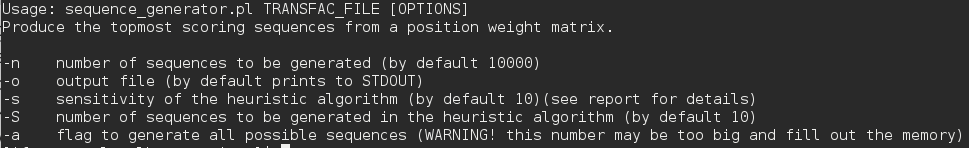
\includegraphics[scale=0.45]{usage.png}
\end{figure}

As can be seen in the picture, there are two options that require no value, -a and -o. The first option tells the program to calculate all the possibilities, depending on the input this option may be excrusiantly slow and require a lot of memory. The -o option tells the program to store the output in a file with name INPUTID\_output$Svalue$S\_$nvalue$M.txt if the parameters S and n are specified or INPUTID\_output.txt if the number of possible generated sequences is less than the value specified by $n$.
\section{Results}
\subsection{TP53 motif}
The matrix provided in this first case is quite sparse, which means that the sequences are very conserved and the total number of sequences that can be generated is not very big, in fact this number is 384 in this case. To solve this case it would suffice with brute force enumeration and sorting the results, however our program can be useful if we only want the 10 top-scoring sequences. Below we can find the output of doing \verb|./sequence_generator.pl tp53_motif.txt -n 10|

\begin{table}[h]
\centering
\begin{tabular}{lc}
\multicolumn{1}{c}{Sequence} & Score \\
GGACATGCCCGGGCATGTCC         & 307   \\
GGACATGCCCGGGCATGTCT         & 307   \\
GGACATGCCCGGGCATGTCG         & 302   \\
GAACATGCCCGGGCATGTCC         & 300   \\
GAACATGCCCGGGCATGTCT         & 300   \\
AGACATGCCCGGGCATGTCC         & 298   \\
AGACATGCCCGGGCATGTCT         & 298   \\
GGACATGCCCGGGCATGTTC         & 298   \\
GGACATGCCCGGGCATGTTT         & 298   \\
GGACATGTCCGGGCATGTCC         & 298  
\end{tabular}
\end{table}
\newpage
\subsection{Pax-6 motif} 
Contrary to the previous case, now the matrix barely has any zero so now the number of possibilities is much larger, n=782.757.789.696. This case highlights the necessity of our approach, since the space requirements alone for the generation of such a number of sequences are overwhelming. As before, we present here the first 10 sequences, using \verb|./sequence_generator.pl pax6_motif.txt -n 10 -S 10|
\begin{table}[h]
\centering
\begin{tabular}{lc}
\multicolumn{1}{c}{Sequence} & Score \\
AATTTTCACGCATGAGTTCAC        & 591   \\
AATTTTCACGCATGAATTCAC        & 590   \\
AATCTTCACGCATGAGTTCAC        & 589   \\
AATTTTCACGCTTGAGTTCAC        & 589   \\
AATCTTCACGCATGAATTCAC        & 588   \\
AATTTTCACGCATGAGTTCAT        & 588   \\
AATTTTCACGCTTGAATTCAC        & 588   \\
AATCTTCACGCTTGAGTTCAC        & 587   \\
AATTTTCACGCATGAATTCAT        & 587   \\
AATTTTCACGCATGACTTCAC        & 587  
\end{tabular}
\end{table}
\end{document}